\section{Results}
\subsection{Task-01 Visualization}

\begin{figure}[ht]
    \centering
    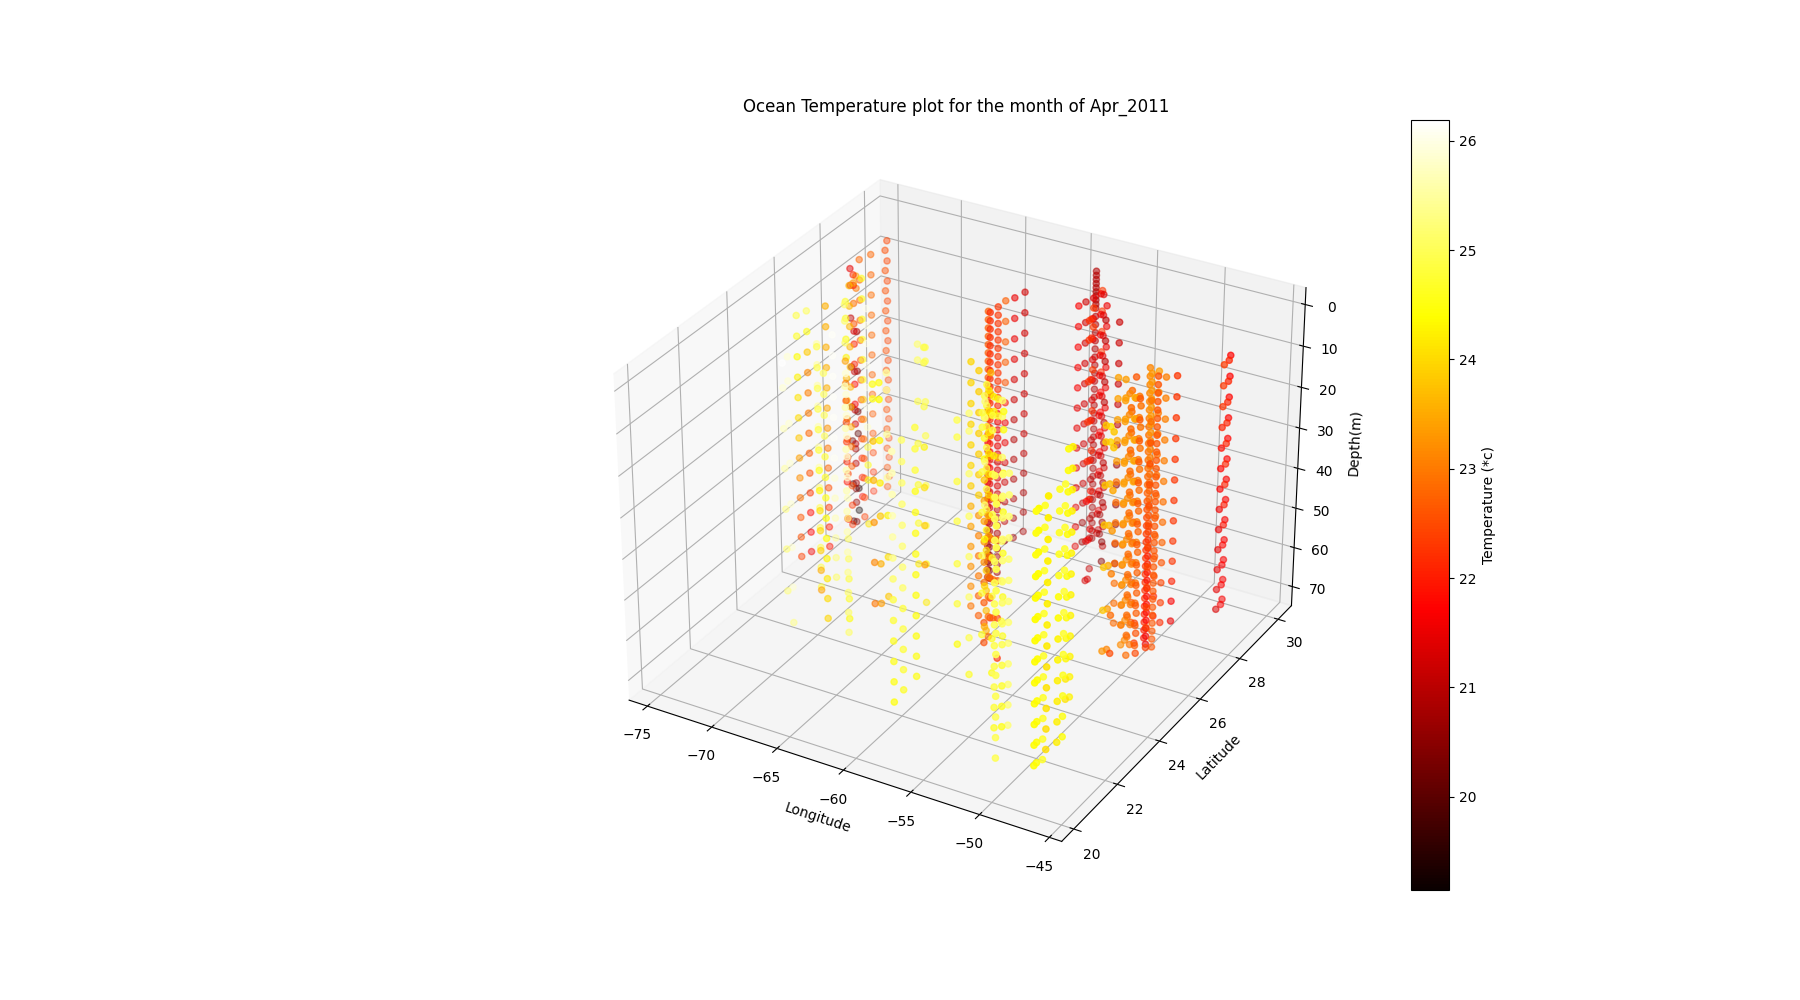
\includegraphics[width = 0.8\linewidth]{figures/oceanTemp.png}
    %\caption{You can cite the source in the caption \cite{xkcd}.}
    %\label{fig:example_1}
\end{figure}

\subsection{Task-02 Visualization}

\begin{figure}[ht] 
  \begin{subfigure}[b]{0.5\linewidth}
    \centering
    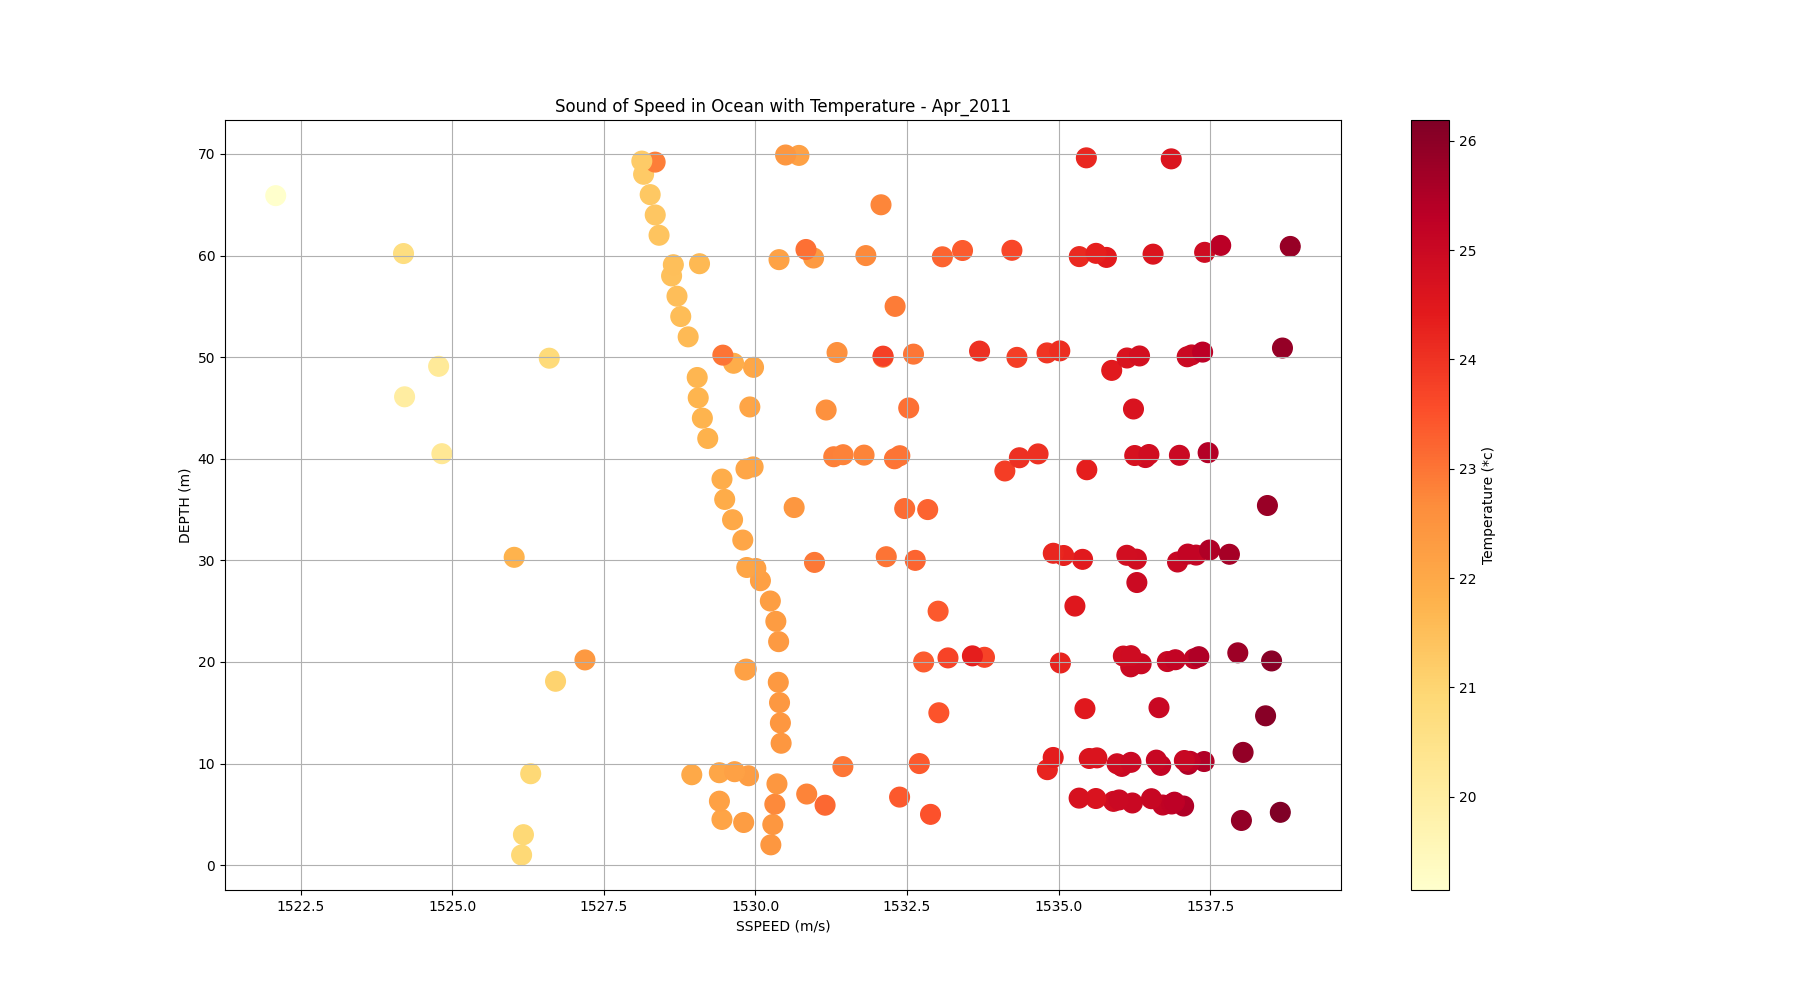
\includegraphics[width=0.9\linewidth]{figures/sspeed_temp.png}
    %\caption{Image a} 
    \label{fig:a} 
    \vspace{4ex}
  \end{subfigure}%% 
  \begin{subfigure}[b]{0.5\linewidth}
    \centering
    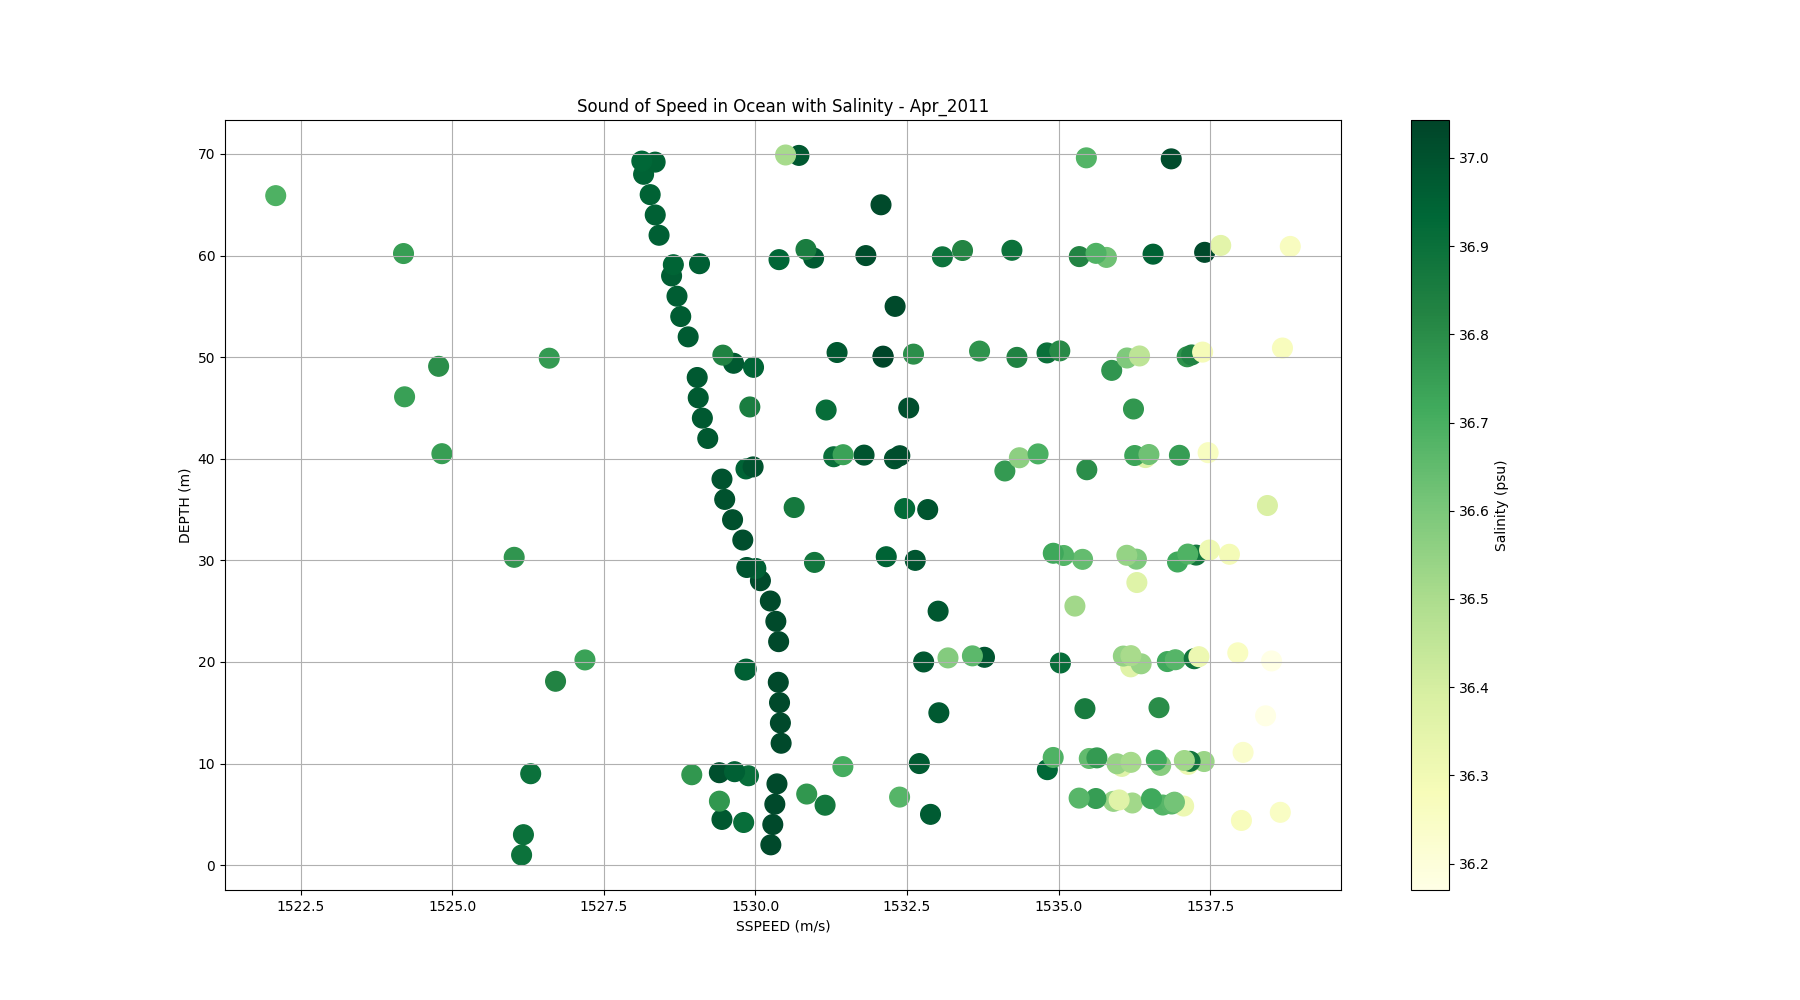
\includegraphics[width=0.9\linewidth]{figures/sspeed_sal.png} 
    %\caption{image b} 
    \label{fig:b} 
    \vspace{4ex}
  \end{subfigure} 
  %\caption{This is how you can create many images at once.}
  %\label{fig:example_many_images} 
\end{figure}

\newpage